% This file was created with tikzplotlib v0.10.1.
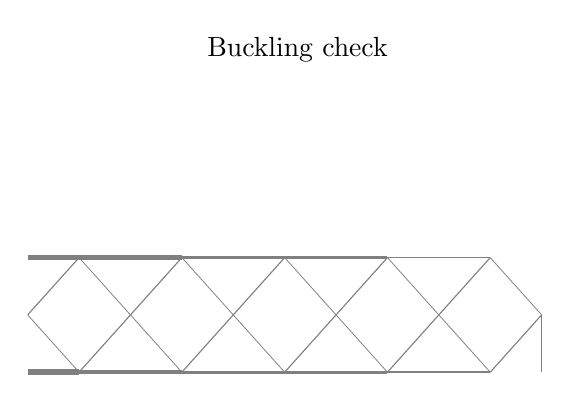
\begin{tikzpicture}

\definecolor{darkgray176}{RGB}{176,176,176}
\definecolor{gray}{RGB}{128,128,128}

\begin{axis}[
hide x axis,
hide y axis,
tick align=outside,
tick pos=left,
title={Buckling check},
x grid style={darkgray176},
xmin=0, xmax=10.5,
xtick style={color=black},
y grid style={darkgray176},
ymin=-2.86209677419355, ymax=4.96209677419355,
ytick style={color=black}
]
\path [draw=gray, line width=2pt]
(axis cs:0,0)
--(axis cs:1,0);

\path [draw=gray, line width=0.282842709403787pt]
(axis cs:1,0)
--(axis cs:0,1);

\path [draw=gray, line width=0.40933068152389pt]
(axis cs:1,0)
--(axis cs:2,1);

\path [draw=gray, line width=0.282842709381618pt]
(axis cs:3,0)
--(axis cs:2,1);

\path [draw=gray, line width=0.409330681530817pt]
(axis cs:3,0)
--(axis cs:4,1);

\path [draw=gray, line width=0.282842709418621pt]
(axis cs:5,0)
--(axis cs:4,1);

\path [draw=gray, line width=0.409330681544904pt]
(axis cs:5,0)
--(axis cs:6,1);

\path [draw=gray, line width=0.282842709463519pt]
(axis cs:7,0)
--(axis cs:6,1);

\path [draw=gray, line width=0.409330681561846pt]
(axis cs:7,0)
--(axis cs:8,1);

\path [draw=gray, line width=0.282842709510371pt]
(axis cs:9,0)
--(axis cs:8,1);

\path [draw=gray, line width=0.409330681584996pt]
(axis cs:9,0)
--(axis cs:10,1);

\path [draw=gray, line width=0.399999997536958pt]
(axis cs:10,0)
--(axis cs:10,1);

\path [draw=gray, line width=0.409330681521052pt]
(axis cs:0,1)
--(axis cs:1,2);

\path [draw=gray, line width=0.28284270937985pt]
(axis cs:2,1)
--(axis cs:1,2);

\path [draw=gray, line width=0.409330681525746pt]
(axis cs:2,1)
--(axis cs:3,2);

\path [draw=gray, line width=0.282842709410086pt]
(axis cs:4,1)
--(axis cs:3,2);

\path [draw=gray, line width=0.409330681534681pt]
(axis cs:4,1)
--(axis cs:5,2);

\path [draw=gray, line width=0.282842709445494pt]
(axis cs:6,1)
--(axis cs:5,2);

\path [draw=gray, line width=0.409330681550351pt]
(axis cs:6,1)
--(axis cs:7,2);

\path [draw=gray, line width=0.282842709494377pt]
(axis cs:8,1)
--(axis cs:7,2);

\path [draw=gray, line width=0.409330681568654pt]
(axis cs:8,1)
--(axis cs:9,2);

\path [draw=gray, line width=0.28284270954286pt]
(axis cs:10,1)
--(axis cs:9,2);

\path [draw=gray, line width=1.99999999999513pt]
(axis cs:0,2)
--(axis cs:1,2);

\path [draw=gray, line width=1.59999999900154pt]
(axis cs:1,0)
--(axis cs:3,0);

\path [draw=gray, line width=1.19999999835686pt]
(axis cs:3,0)
--(axis cs:5,0);

\path [draw=gray, line width=0.973557921236028pt]
(axis cs:5,0)
--(axis cs:7,0);

\path [draw=gray, line width=0.688409406411637pt]
(axis cs:7,0)
--(axis cs:9,0);

\path [draw=gray, line width=1.59999999899368pt]
(axis cs:1,2)
--(axis cs:3,2);

\path [draw=gray, line width=1.19999999834929pt]
(axis cs:3,2)
--(axis cs:5,2);

\path [draw=gray, line width=0.799999997705747pt]
(axis cs:5,2)
--(axis cs:7,2);

\path [draw=gray, line width=0.399999997066403pt]
(axis cs:7,2)
--(axis cs:9,2);

\end{axis}

\end{tikzpicture}
